\section{Calibration}
\label{sec:calib}
The accuracy of simulated events is evaluated with data taken while a
radioactive source was deployed within the detector volume.
For this analysis an $\ce{^{16}N}$ source was used.
The SNO+ $\ce{^{16}N}$ source was developed for SNO, as
their primary energy calibration source~\citep{sno_n16}.
The methods and results of SNO+'s $\ce{^{16}N}$ calibration are summarized here but
are described in greater detail by~\citep{snop_water_unidoc}.

\begin{figure}[htbp]
\centering
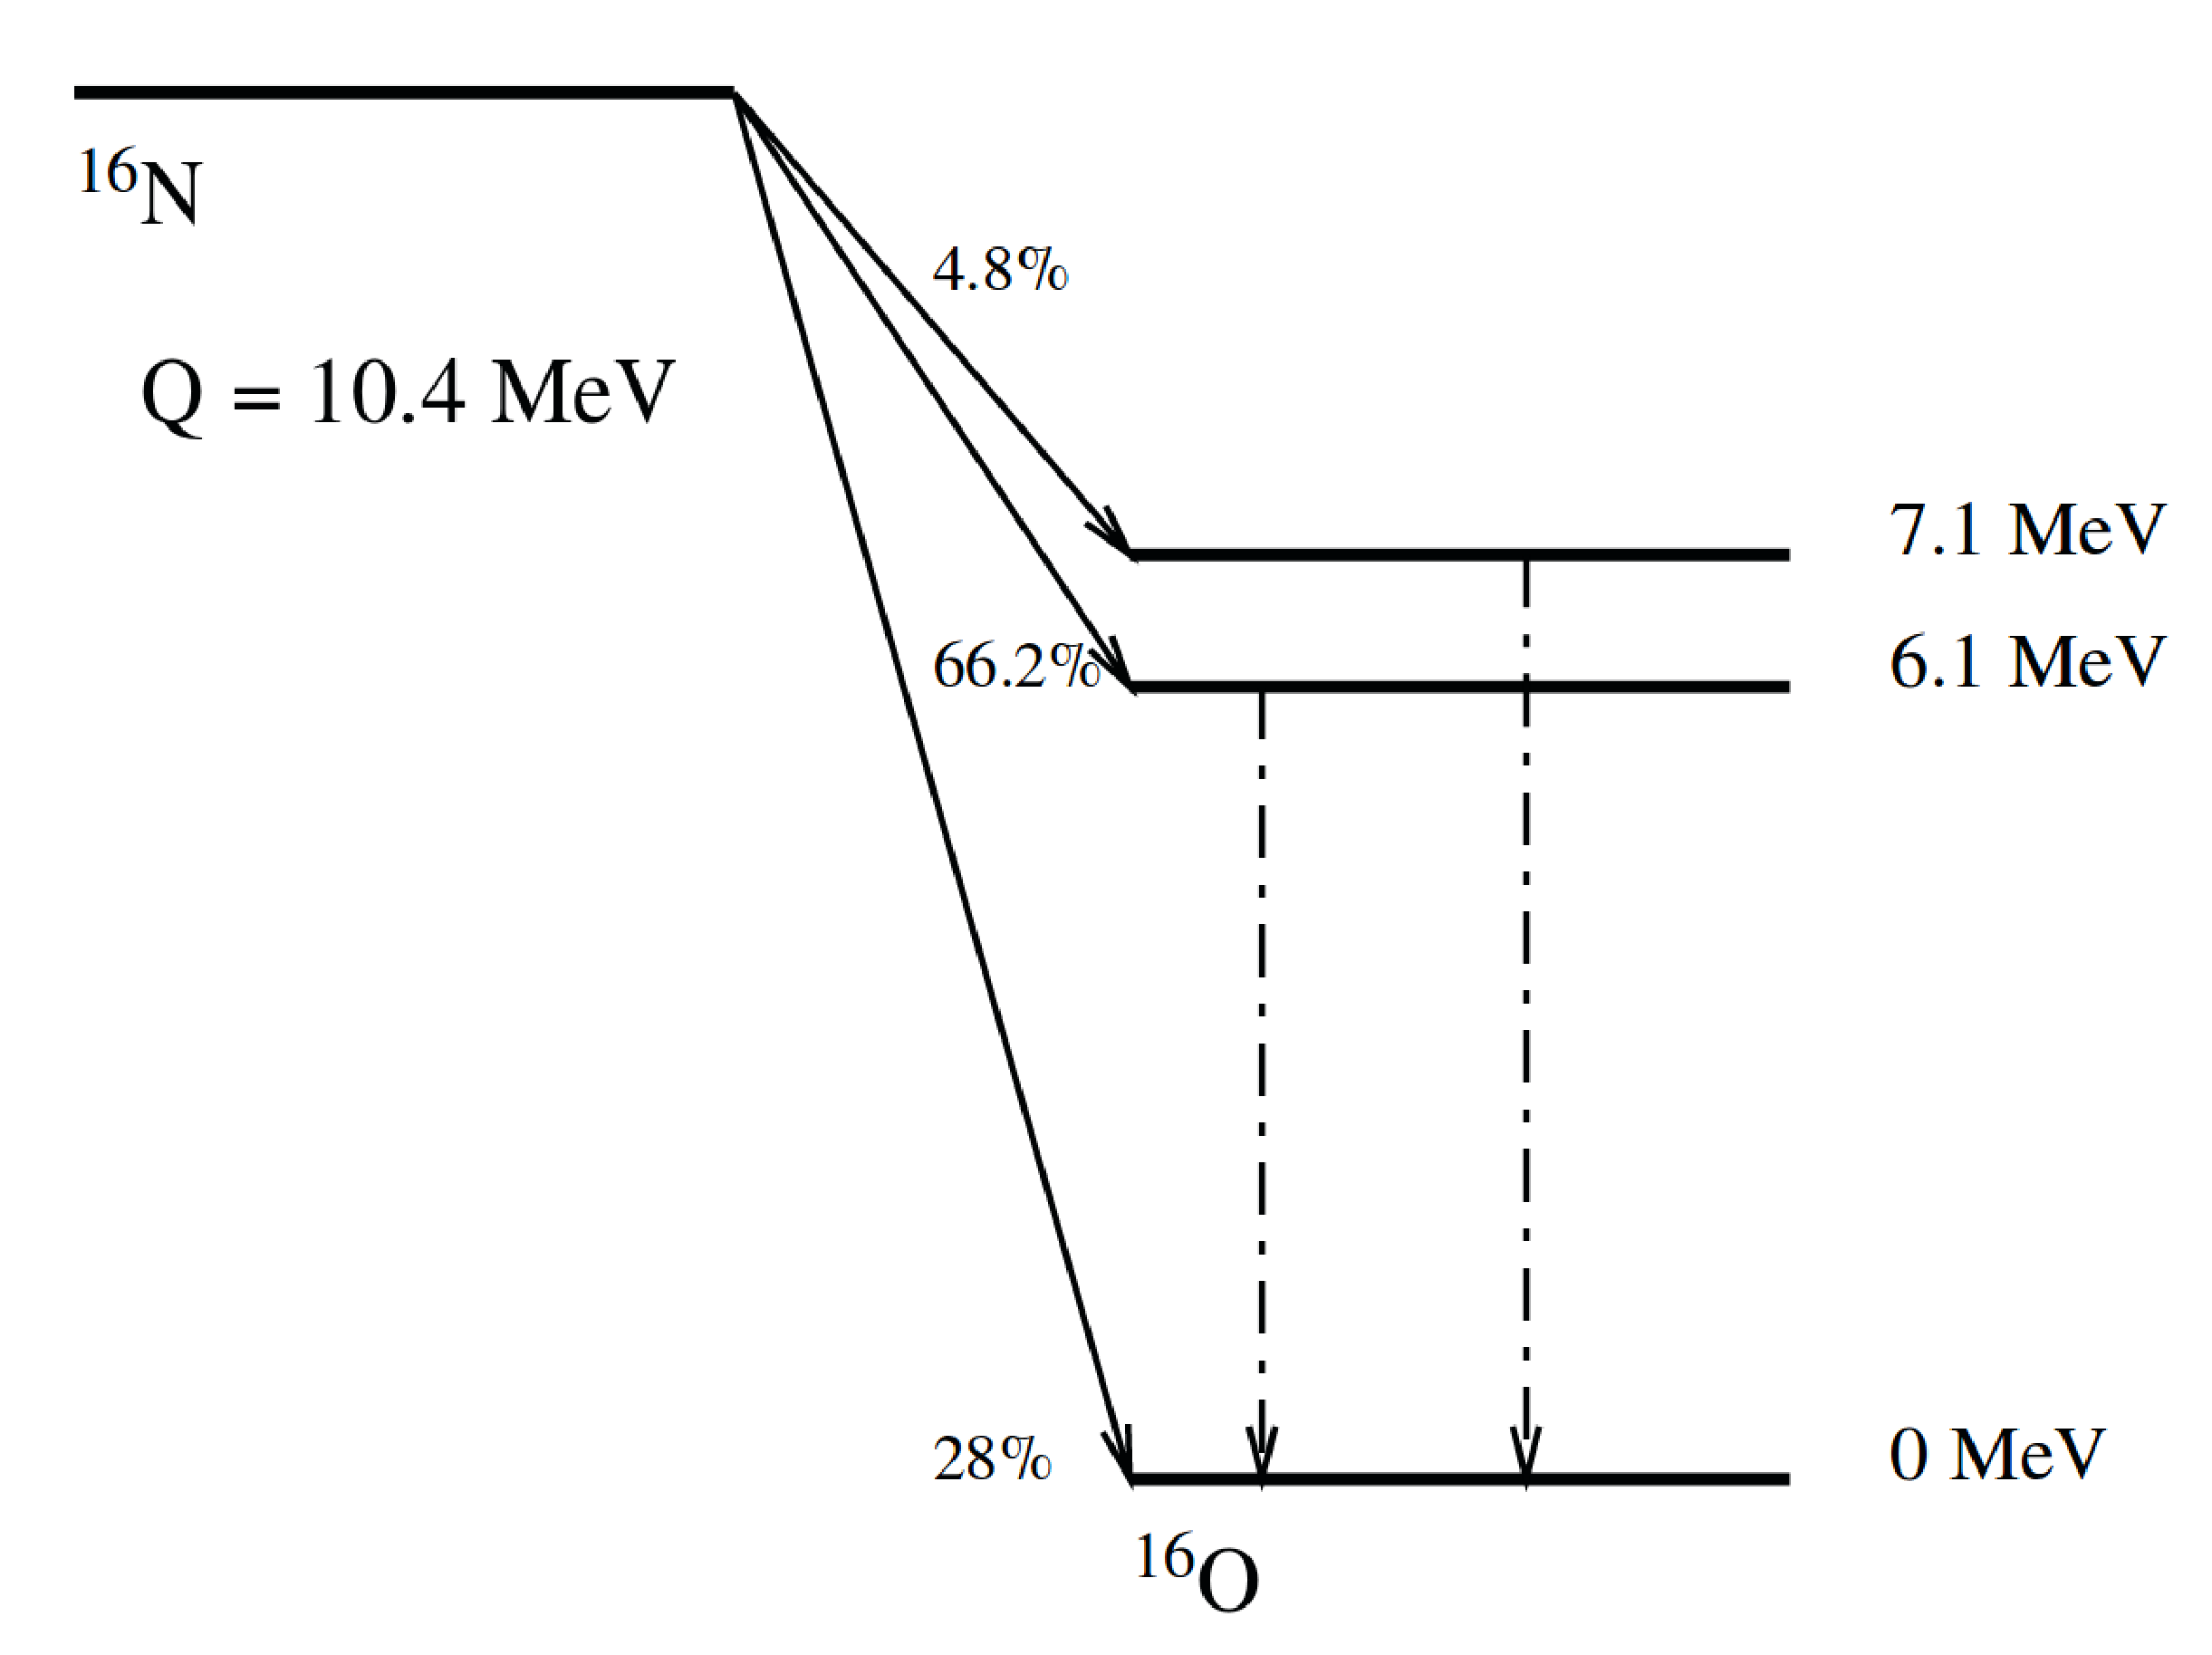
\includegraphics[width=0.58\textwidth]{n16_branching_ratios}
\caption[Major $\ce{^{16}N}$ Branching Ratios]{The most significant branching ratios for $\ce{^{16}N}$ decaying
to an excited state of $\ce{^{16}O}$. Figure from~\cite{sno_n16}.}
\label{fig:n16_br}
\end{figure}
The $\ce{^{16}N}$ source was developed by SNO, it uses a commercial
deuterium and tritium generator (DT-generator) to produce gaseous $\ce{^{16}N}$.
The gas is pumped into the deployed source where it can undergo $\beta$-decay
to an excited state of $\ce{^{16}O}$, the $\ce{^{16}O}$ will then de-excite
and typically emit a $6.1$\,MeV gamma particle. Higher or lower energy gammas are emitted
at a lower rate, the branching ratios for the de-excitation gammas are shown in
Fig~\ref{fig:n16_br}.

A small block of plastic scintillator, observed by a PMT, is embedded within the
source cannister. The PMT detects the $\beta$ from the initial
$\ce{^{16}N} \rightarrow \ce{^{16}O^{*}}$ decay. That PMT signal is used as a
tag in the detector DAQ to identify events from the deployed source.

The source position within the AV was varied in a 3-dimensional
scan.
A 1-dimensional scan was done along the z-axis between the AV and PSUP\@.
Scanning many positions allowed for a position dependent evaluation of
systematics and a position dependent correction to the reconstructed energy.

\subsection{Energy Calibration}
The detector resolution $\sigma_{E}$ and relative energy scale $\delta_{E}$ are determined
from the $\ce{^{16}N}$ energy spectrum.
The energy spectrum is modeled by $P(T_\mathrm{e})$, the energy spectrum in
electron equivalent kinetic energy, and is given by $P_{\mathrm{source}}(T_{\mathrm{e}})$
convolved with a normalized Gaussian distribution,
\begin{equation}
    P(T_\mathrm{e}) = N \int P_\mathrm{source}(T^{\prime}_{e})\frac{1}{\sqrt{2\pi}\sigma_{E}}e^-{\frac{\left((1+\delta_E)T_\mathrm{e}-T^{\prime}_{e}\right)^{2}}{2\sigma^{2}_{E}}}dT^{\prime}_{e}\text{.}%-\Delta E
\label{eq:convolution}
\end{equation}
$P_\mathrm{source}(T_{\mathrm{e}})$ represents the distribution of deposited energy in
the detector from the $\ce{^{16}N}$ source, in electron equivalent energy.
Since the $\ce{^{16}N}$ emits gammas into the detector the mapping between
gamma energy and electron equivalent energy is done by finding the electron
energy that can produce the same number of Cherenkov photons
as each gamma; this is not a one-to-one mapping because the same electron or gamma
energy will not always produce the same number of photons.
The mapping is determined from simulation and is shown in
Fig.~\ref{fig:cherenkov_energy_map}.
The gamma to electron energy mapping is then applied to the simulated $\ce{^{16}N}$
gamma energy spectrum to determine $P_\mathrm{source}(T_{\mathrm{e}})$.

\begin{figure}[htbp]
\centering
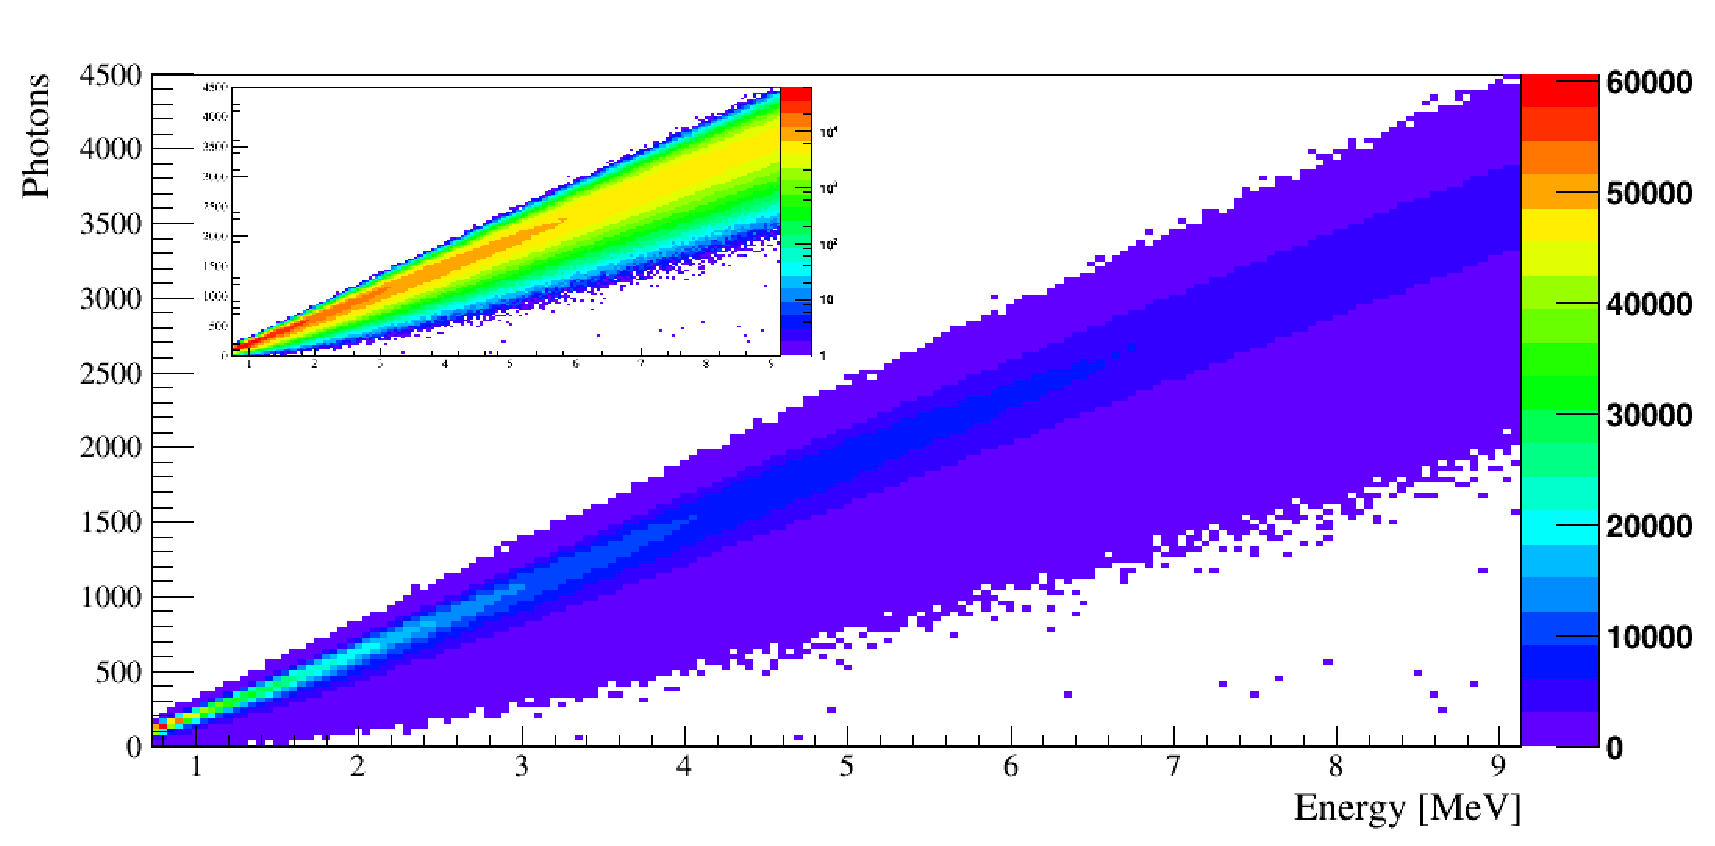
\includegraphics[width=0.78\textwidth]{cherenkov_nhit_energy_map.eps}
\caption[Electron Cherenkov Photon Product PDF]{ The map between electron
energy and expected Cherenkov photons production.  Used for the energy
calibration to map between gamma energy and equivalent electron energy.  This is
the same PDF used by EnergyRSP to estimate energy from the observed PMT hits.}
\label{fig:cherenkov_energy_map}
\end{figure}

\begin{figure}[htbp]
\centering
\begin{subfigure}{0.48\textwidth}
\centering
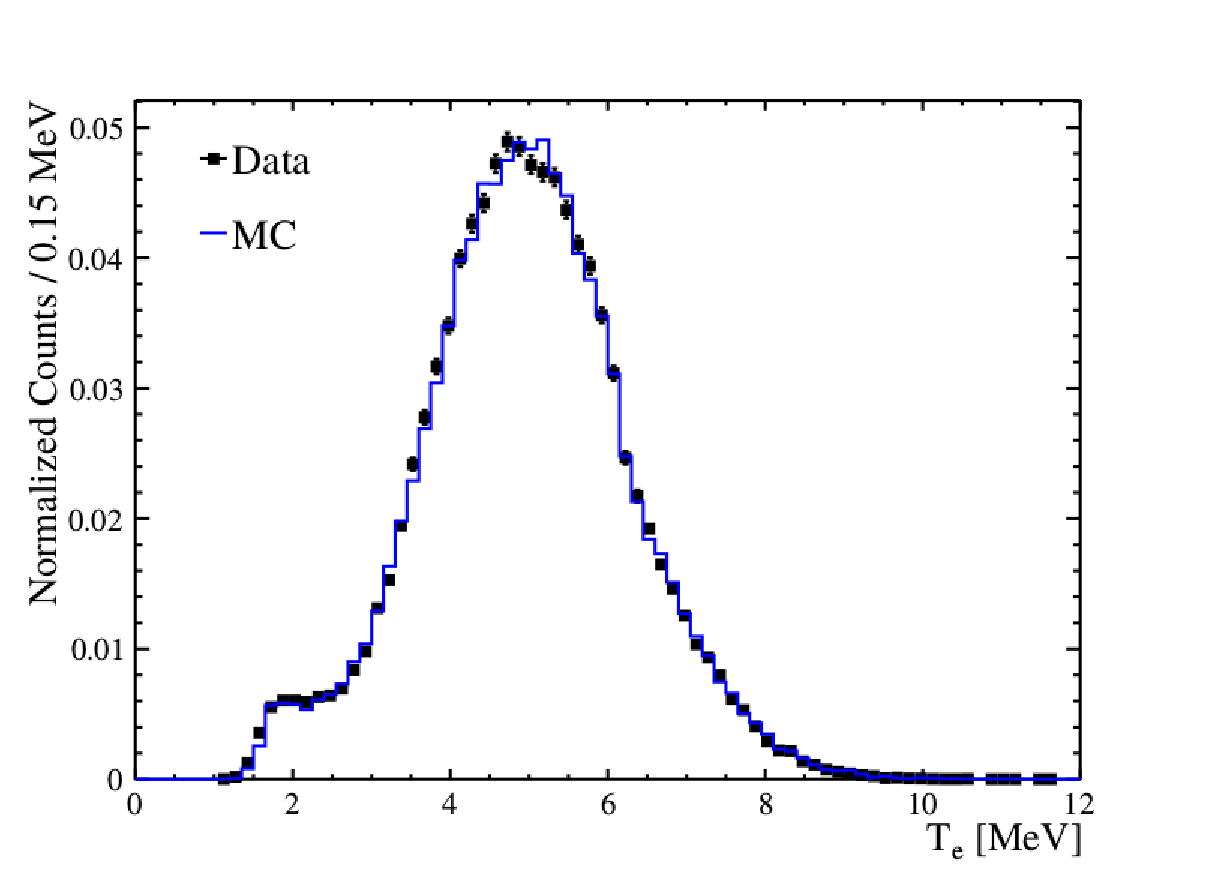
\includegraphics[width=\textwidth]{energy_data_vs_mc}
\caption[]{}
\end{subfigure}
\hfill
\begin{subfigure}{0.48\textwidth}
\centering
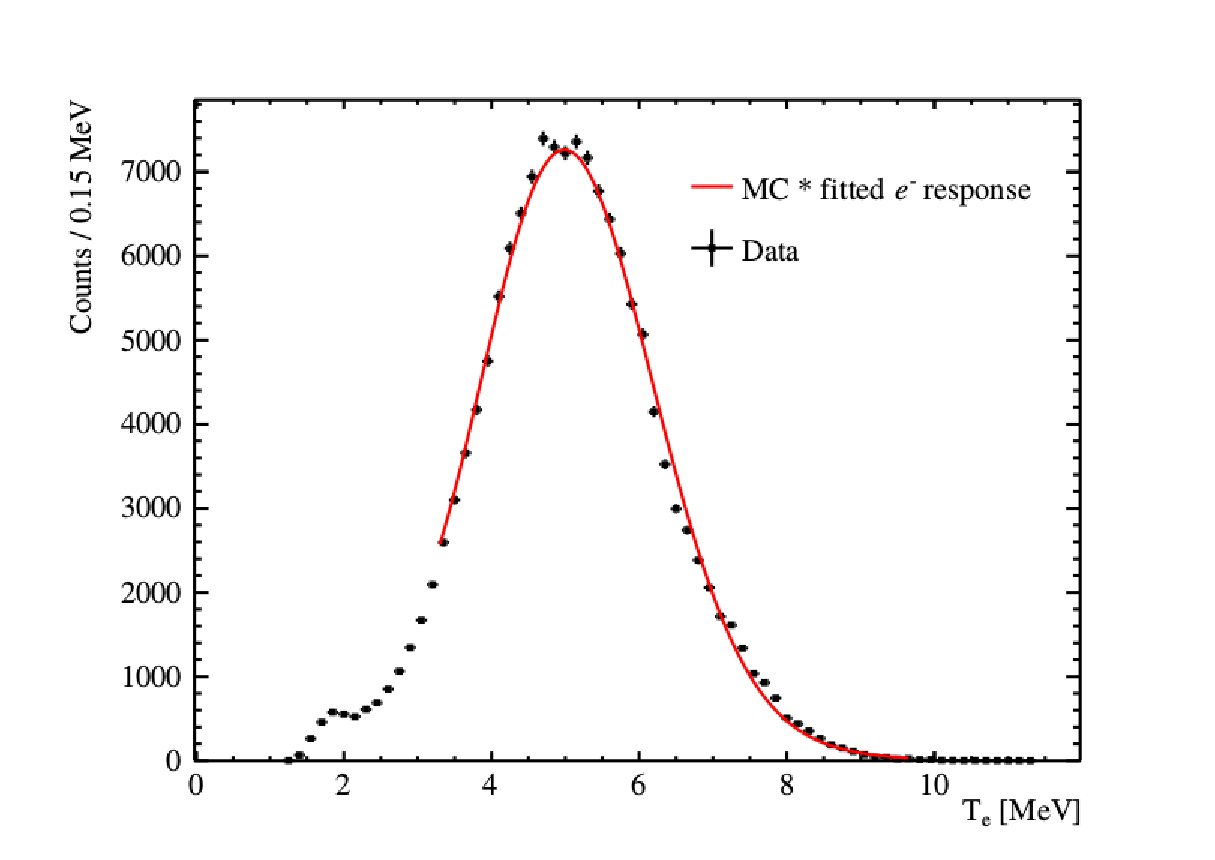
\includegraphics[width=\textwidth]{N16energyFit}
\caption[]{}
\end{subfigure}
\caption[$\ce{^{16}N}$ Energy Comparisons]{ (a) The comparison between
reconstructed energy for $\ce{^{16}N}$ data and monte-carlo.  (b) Fit of
Eqn.~\eqref{eq:convolution} to distribution of reconstructed energies for
detected central $\ce{^{16}N}$ events.}
\label{fig:n16_energy}
\end{figure}
The values for $\sigma_{E}$ and $\delta_{E}$ are extracted from~\eqref{eq:convolution}
by performing a fit to the reconstructed $\ce{^{16}N}$ energy spectrum.
The fit is done to both simulated $\ce{^{16}N}$ data and to detector data,
each determining their own values for $\sigma_{E}$ and $\delta_{E}$.
As is show in Fig~\ref{fig:n16_energy}, this fit is only performed
over the energy range $3.25$ to $9.6$\,MeV, at energies outside this range
difficult to model source-container effects dominate the energy spectrum.
It's worth noting that $\sigma_{E}$ represents only the resolution provided by detector
effects, resolution from effects such as photon statistics are accounted
for in $P_\mathrm{source}(T_{\mathrm{e}})$.

Values for $\sigma_{E}$ and $\delta_{E}$ are extracted for data taken, or simulated, with
the $\ce{^{16}N}$ source at many position, allowing for a position dependent
determination of the energy scale and resolution.
Fitting to both simulated and to detected data allows for a correction to
be created that can make the two datasets match better, however the data
used to create the correction cannot then be used to determine systematics.
So the $\ce{^{16}N}$ data was split into two datasets, one for determining
what correction should be applied to simulation, the other for extracting systematics
after the correction is applied.

The data for the correction is further divided into position bins in $z$ and
$\rho$, where $\rho = \sqrt{x^{2} + y^{2}}$. The choice of binning is motivated
by the symmetry of the detector, the detector is very symmetric for an interchange
of $x$ and $y$ or $x,y \rightarrow -x,-y$.
There exists, however, significant asymmetries along the $z$ axis
from the detector neck and from the rope-net along the top of the AV\@.
The data is divided into 4-bins along the $\rho$ direction each $200$\,cm long
and bins of $57$\,cm height along the $z$ axis. The number of bins along the
z-axis varies for each slice in $\rho$ because data was primarily taken within
the AV.\@
Figure~\ref{fig:n16_uniformity} shows position dependence of the fits for
$\delta_{E}$ and $\sigma_{E}$ in each bin for both simulated and detected
events.

\begin{figure}[htbp]
\centering
\begin{subfigure}{0.49\textwidth}
\centering
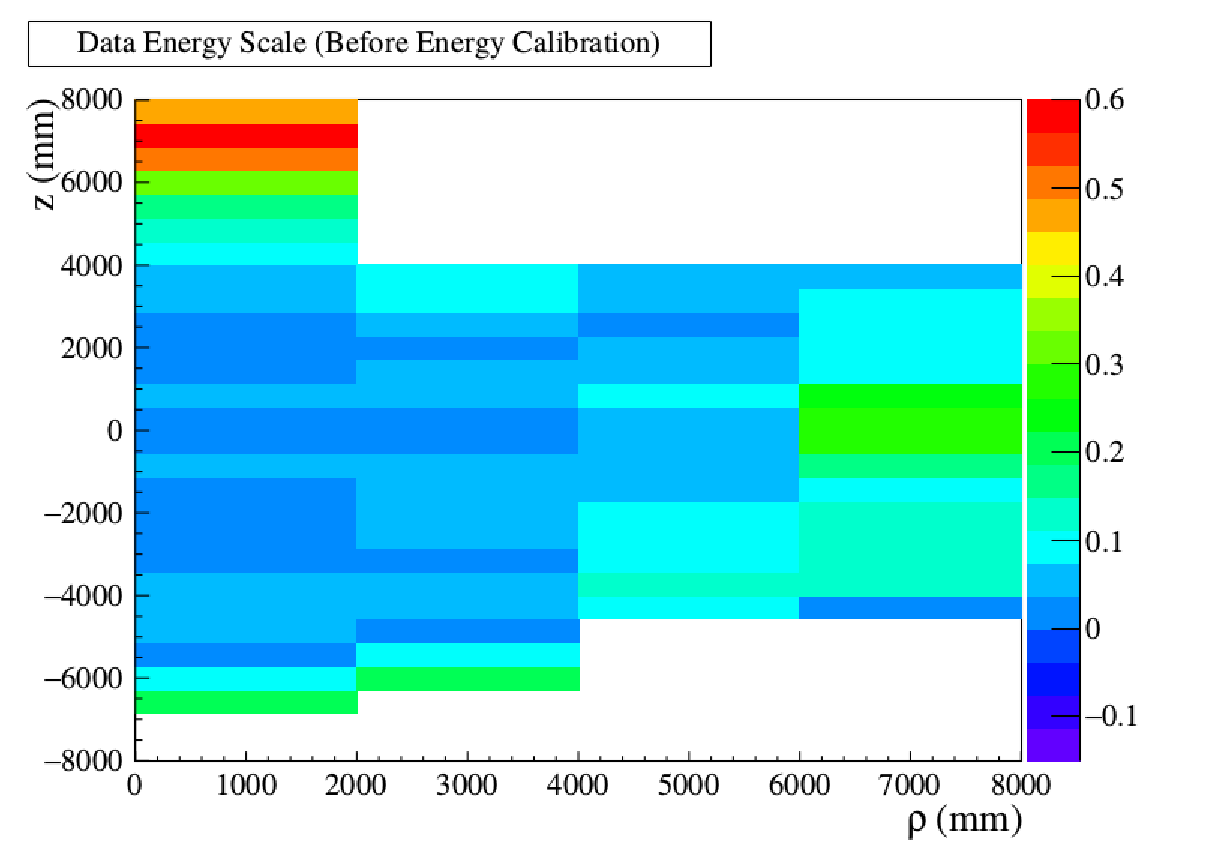
\includegraphics[width=\textwidth]{data_scale_uniformity}
\caption[]{}
\end{subfigure}
\hfill
\begin{subfigure}{0.49\textwidth}
\centering
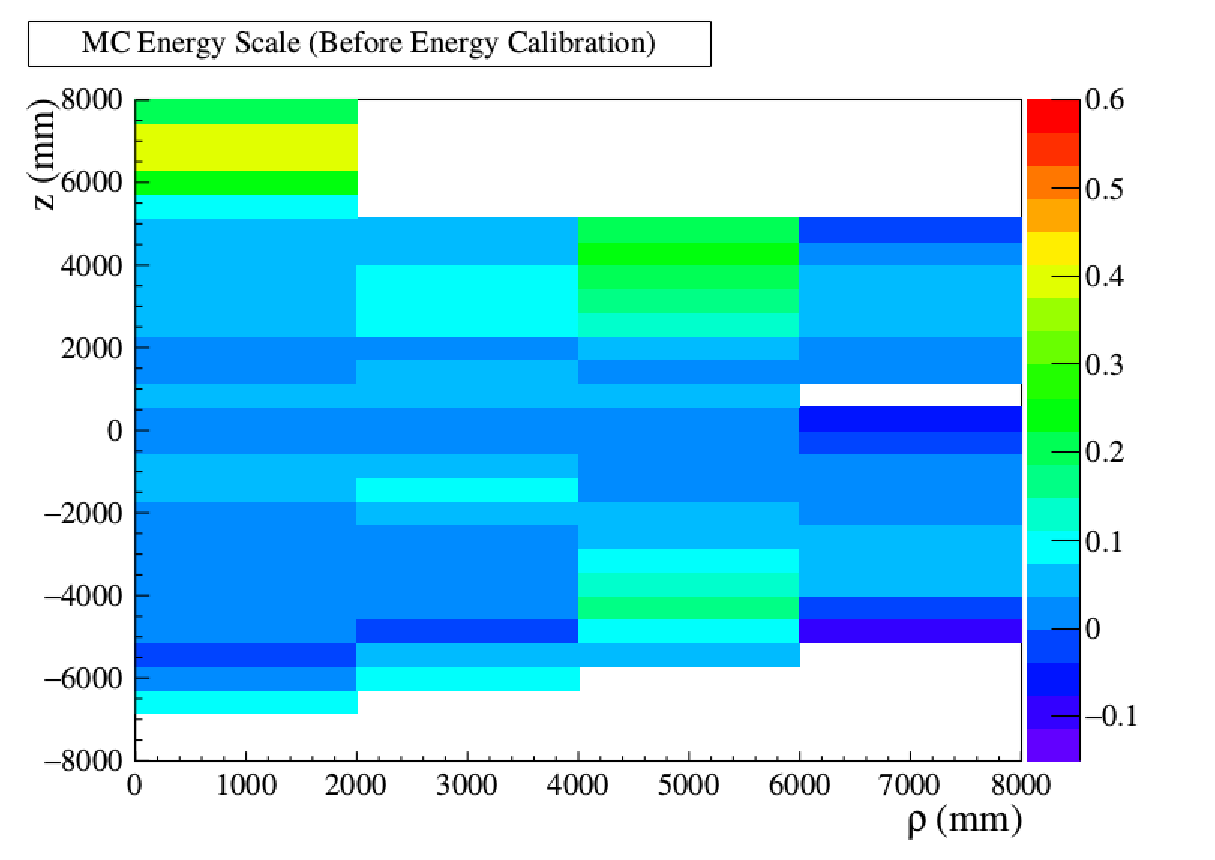
\includegraphics[width=\textwidth]{mc_scale_uniformity}
\caption[]{}
\end{subfigure}

\begin{subfigure}{0.49\textwidth}
\centering
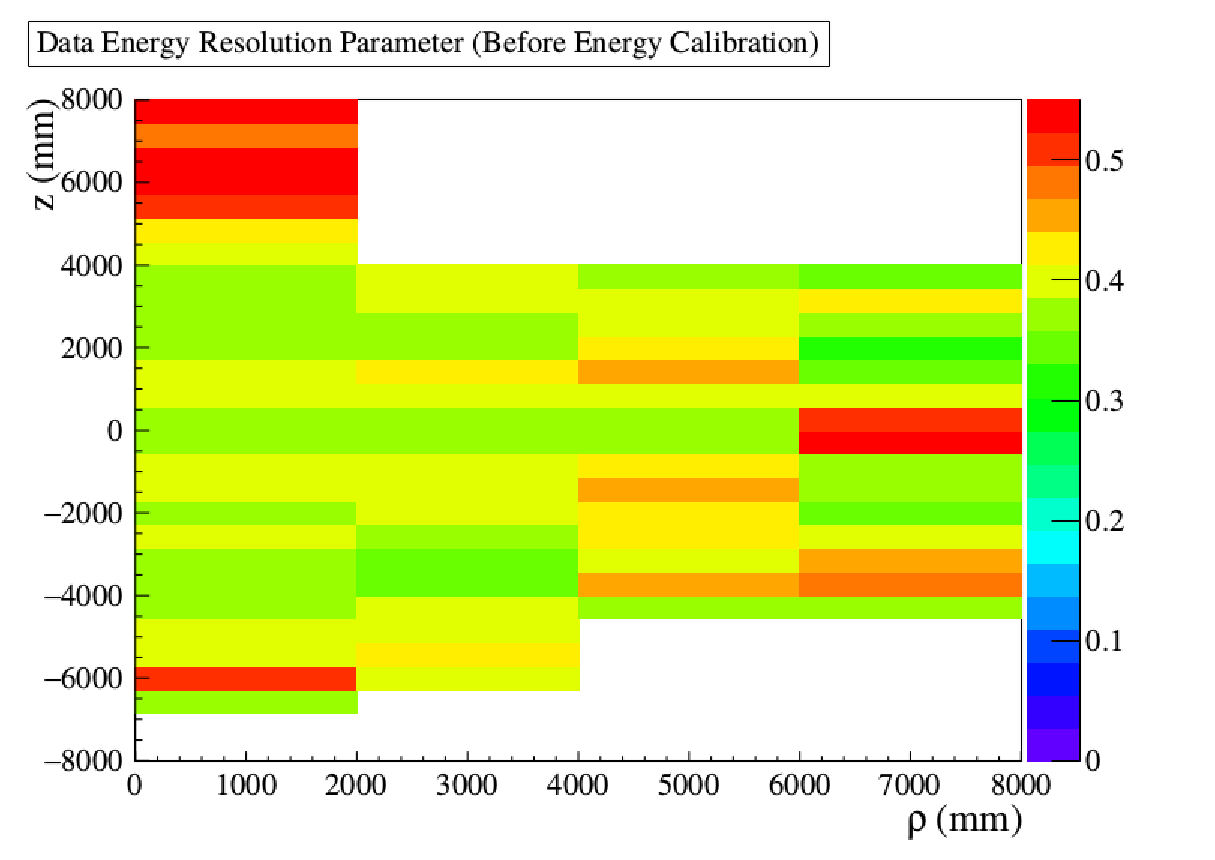
\includegraphics[width=\textwidth]{data_sig_uniformity}
\caption[]{}
\end{subfigure}
\hfill
\begin{subfigure}{0.49\textwidth}
\centering
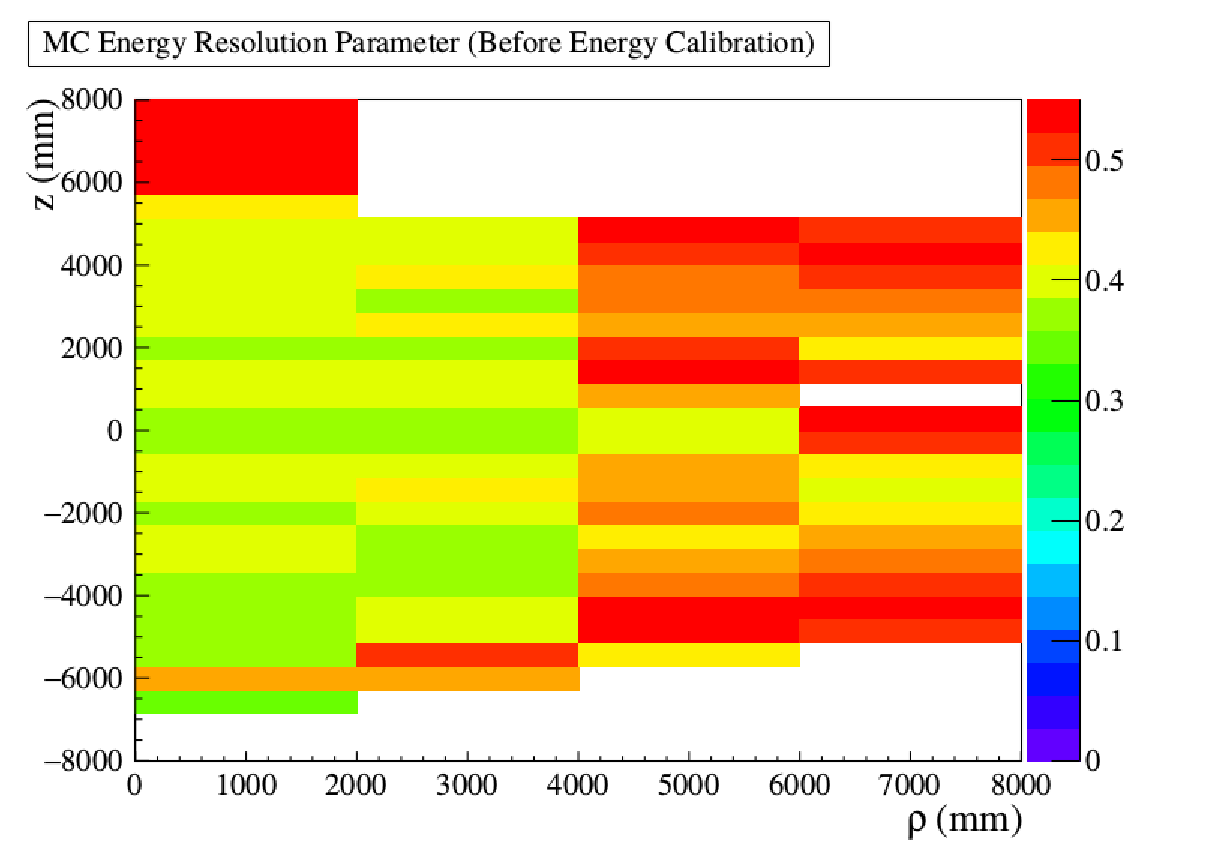
\includegraphics[width=\textwidth]{mc_sig_uniformity}
\caption[]{}
\end{subfigure}
\caption[Position Depedence of Energy Scale and Resolution from $\ce{^{16}N}$]
{The best fit energy scale before for detected (a) and monte-carlo simulated (b)  $\ce{^{16}N}$
events as a function of position.
And the best fit energy resolution parameter for detected (c) and 
simulated (d) $\ce{^{16}N}$ events}
\label{fig:n16_uniformity}
\end{figure}

\begin{figure}[htbp]
\begin{subfigure}{0.49\textwidth}
\centering
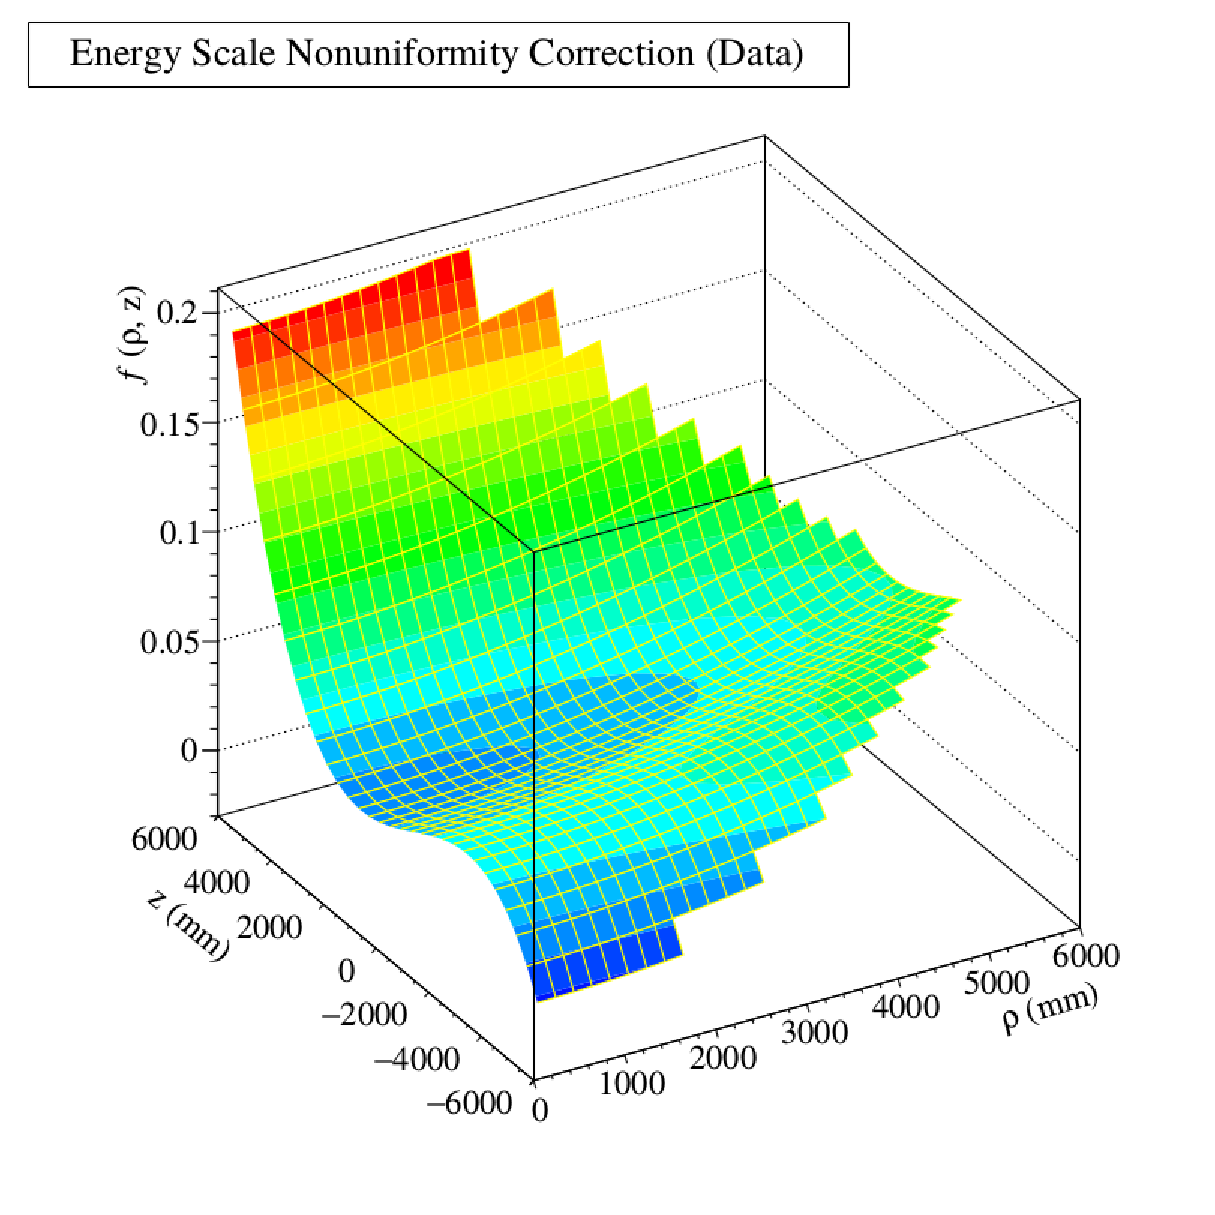
\includegraphics[width=\textwidth]{energy_uniformity_correction}
\caption[]{}
\end{subfigure}
\hfill
\begin{subfigure}{0.49\textwidth}
\centering
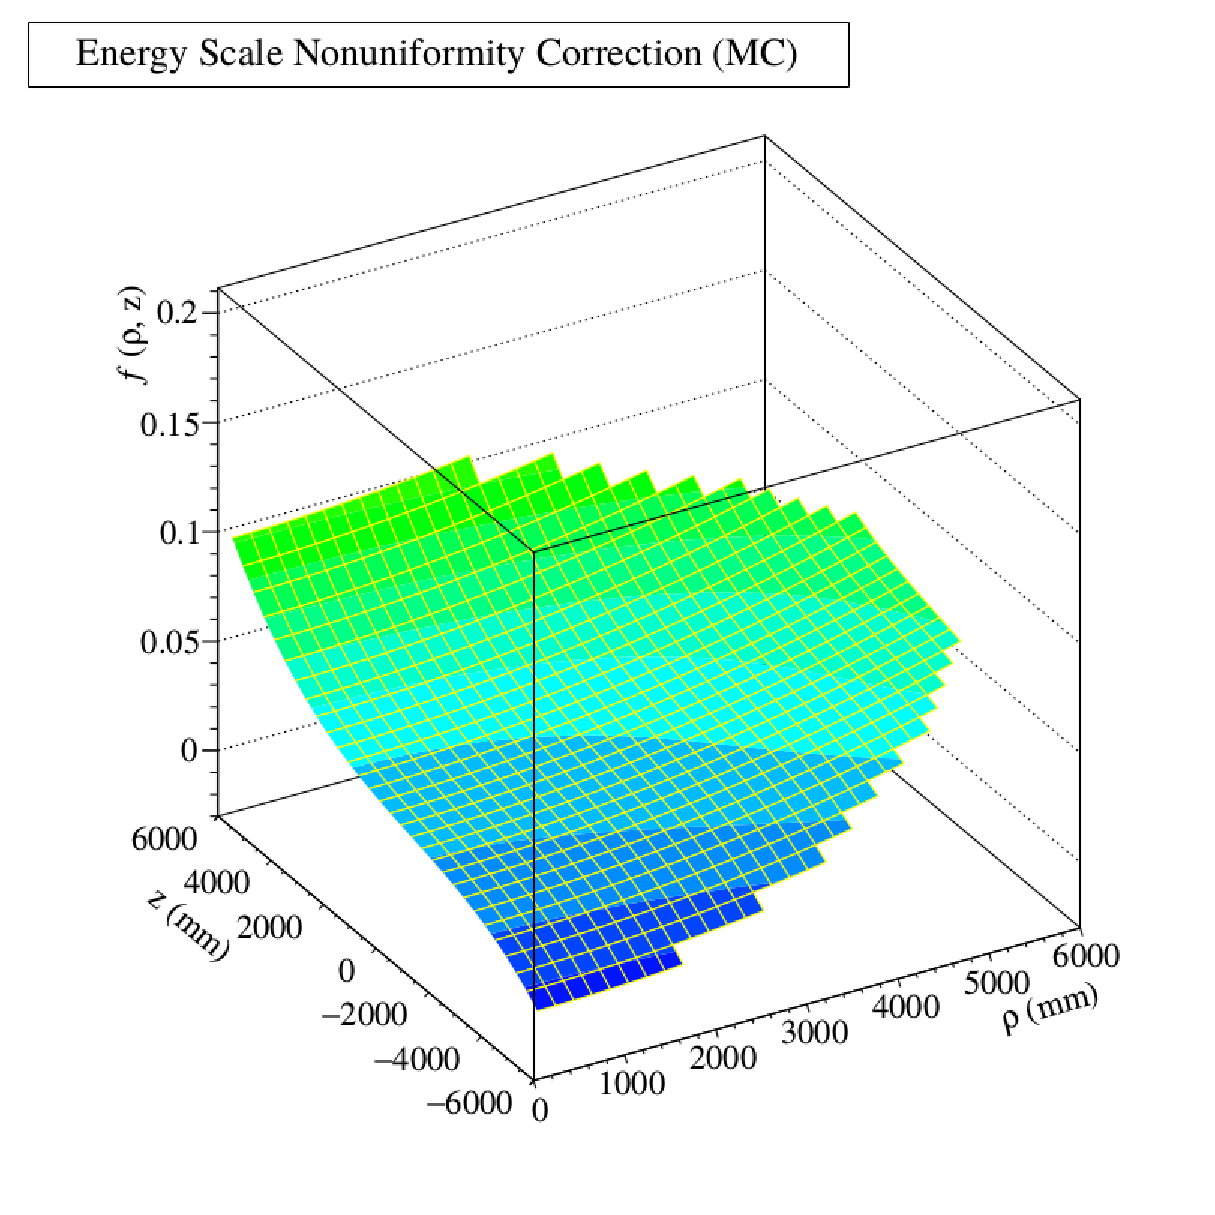
\includegraphics[width=\textwidth]{energy_mc_uniformity_correction}
\caption[]{}
\end{subfigure}

\begin{subfigure}{0.49\textwidth}
\centering
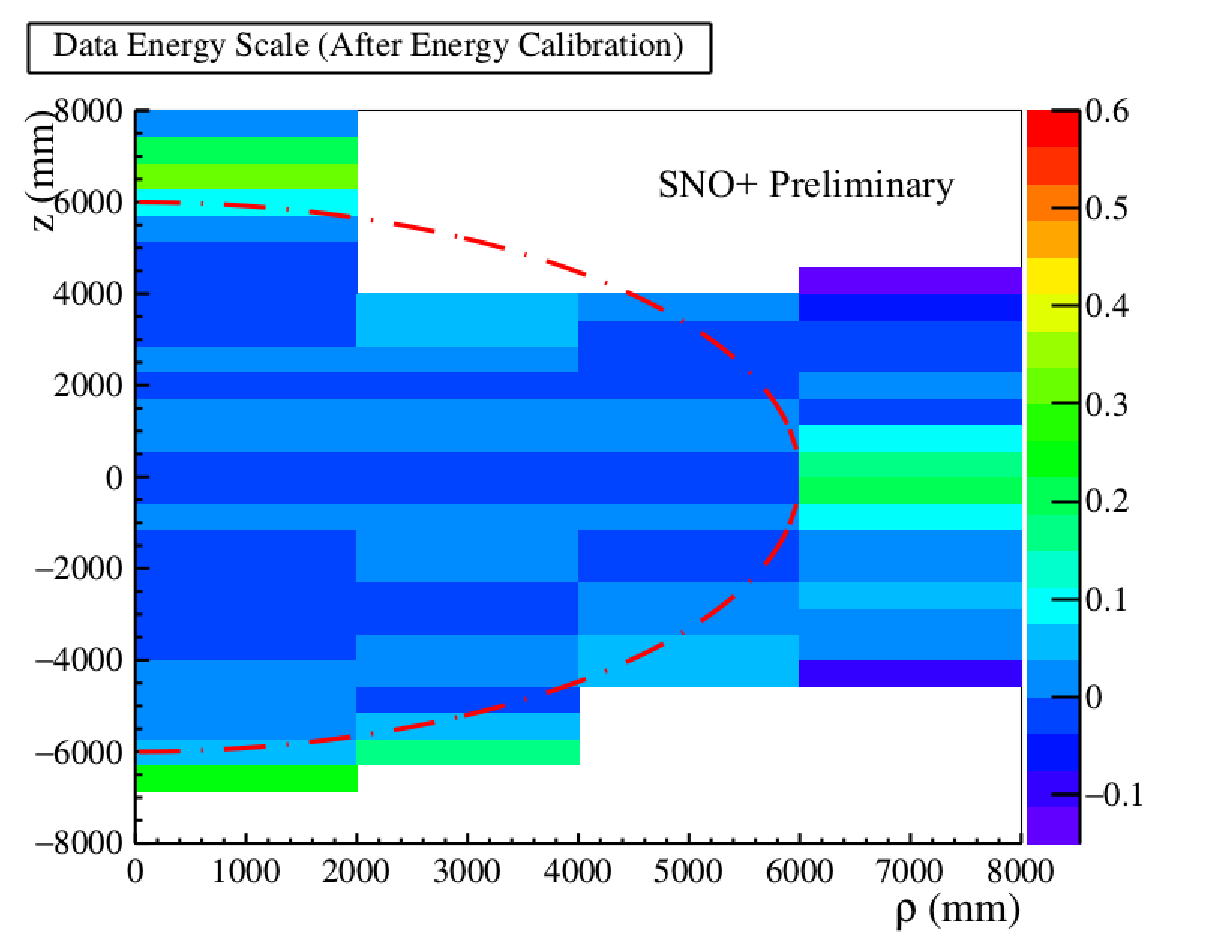
\includegraphics[width=\textwidth]{Res_data}
\caption[]{}
\end{subfigure}
\hfill
\begin{subfigure}{0.49\textwidth}
\centering
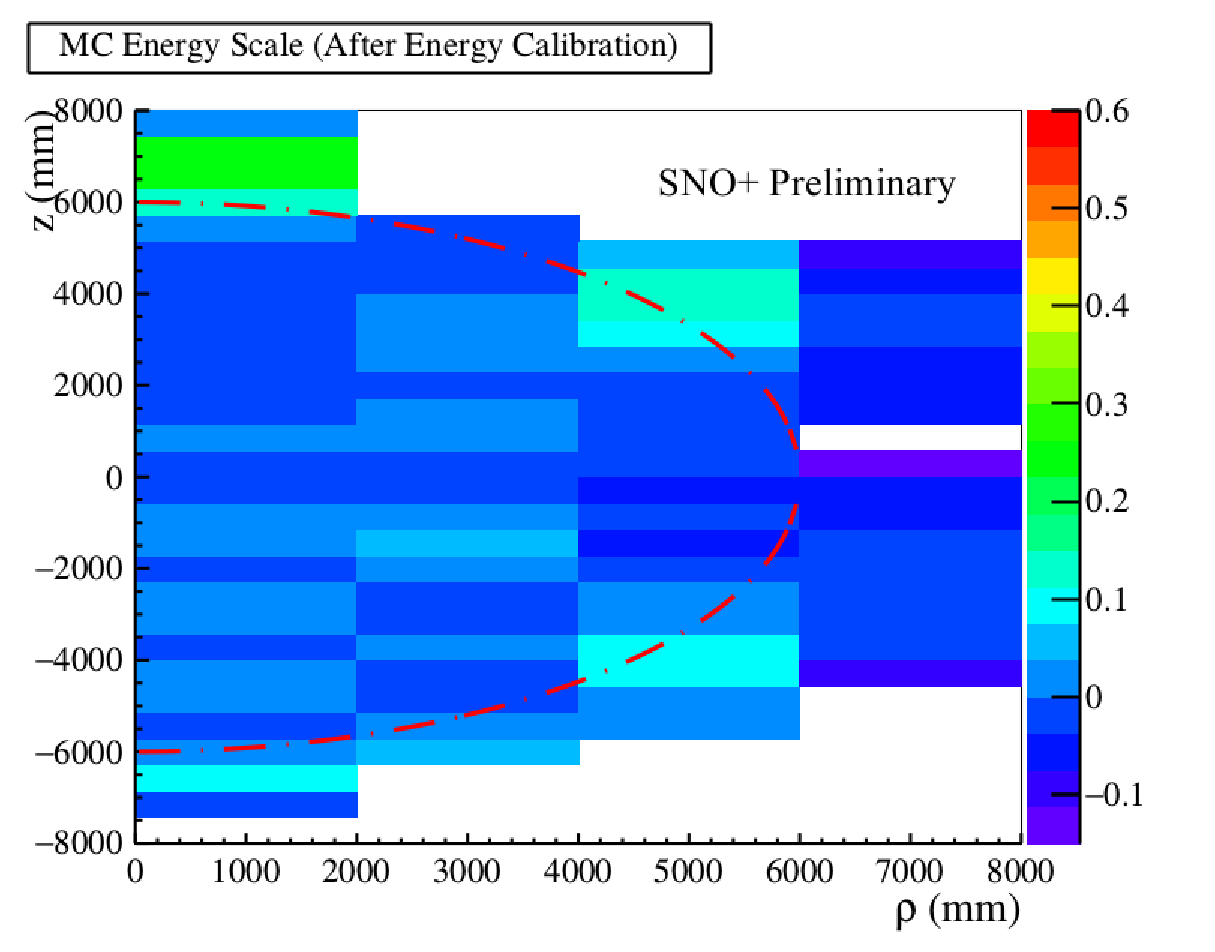
\includegraphics[width=\textwidth]{Res_MC}
\caption[]{}
\end{subfigure}
\caption[Energy Scale Uniformity Correction and Results]{The energy scale
non-uniformity correction for data (a) and MC simulation (b).
The measured energy scale as a function of position after the application
of the non-uniformity correction for data (c) and MC simulation (d).}
\label{fig:uniformity_corrections}
\end{figure}

Variations in $\delta_{E}$ along $z$ and $\rho$ were modeled by a polynomial given by,
\begin{equation}
    \delta_{E}(\rho^{2}, z) = A + \left[(1+B\rho^{2})(1+Cz+Dz^{2}+Ez^{3}) - 1\right]\text{.}
    \label{eqn:escale_position_dependence}
\end{equation}
Values for $A$, $B$, $C$, $D$, and $E$ are extracted from a fit to the observed
spatial variation of $\delta_{E}$ for simulation and data and are given in
table~\ref{tbl:n16_position_escale}.
The reconstructed energies of simulated and detected 
events are then corrected according to~\eqref{eqn:escale_position_dependence} by
their respective best fit values.
Figure~\ref{fig:uniformity_corrections} shows the correction as a function of
position in the detector and the energy scale measured across the detector
after the application of the correction.
The energy resolution is evaluated as a function of position but no correction
is determined from it.
\begin{table}
    \centering
\begin{tabular}{|c | c | c | c |c|c|}
\hline
& A&B&C&D&E\\
\hline
Data& 2.53e-2& 1.48-e9 & -5.44e-6 & 2.14e-9 & 6.49e-13\\
Simulation& 3.33e-2& 9.48e-10& 3.77e-6& 4.46e-10& 1.43e-13\\
\hline
\end{tabular}
\caption{Best fit values for~\eqref{eqn:escale_position_dependence} for
simulated and detected data, determined using units of mm for $z$ and $\rho$.}
\label{tbl:n16_position_escale}
\end{table}

After the correction is applied to remaining half of the calibration dataset
$\sigma_{E}$ and $\delta_{E}$ are determined once more as a function of position.
The bin-by-bin differences in $\sigma_{E}$ and $\delta_{E}$ between
simulated and detected data are taken as the systematic uncertainty for those
parameters, with additional fit uncertainties added in quadrature.
Averaging the bin-by-bin systematic uncertainty over the detector volume relevant
for the solar analysis yields a $2.5\%$ uncertainty on $\delta_{E}$ and an
$11\%$ uncertainty on $\sigma_{E}$.

\subsection{Position Calibration}
Similar to the energy calibration, the position reconstruction is evaluated
using $\ce{^{16}N}$ data and simulation.
The difference between the source position and the reconstructed
position of each event is determined and histogrammed.
A fit to that distribution is performed using a model of a Gaussian distribution
with exponential tails convolved with a distribution for the first gamma interaction
distance. The equation for this is given by,
\begin{equation}
    P(x)  = A \cdot \bigg[ \bigg(\frac{1 - \alpha}{\sqrt{2\pi}\sigma}e^{- \frac{(x-\mu)^2}{2\sigma^2}} + \frac{\alpha }{2 \tau}e^{-\frac{|x-\mu|}{\tau}}\bigg) \circledast P_{\gamma}(x) \bigg]\text{.}
    \label{eqn:n16_position_model}
\end{equation}
Where $\mu$ and $\sigma$ are respectively the center and width of the Gaussian,
$\tau$ represents the decay rate for the exponential tails, and $\alpha$ represents
the relative strength of the exponential~vs.~the Gaussian;
$P_{\gamma}(x)$ is distribution of distance travelled by an $\ce{^{16}N}$
gamma before it's first interaction, it is determined from a separate MC
simulation.
Finally $A$ is an overall normalization to account for the number of events
included in the distribution.
The Gaussian and exponential portion of
\eqref{eqn:n16_position_model} represents the spread introduced by the detector
and position reconstruction, the $P_\gamma$ term represents the intrinsic spread
in interaction positions from the source itself.
The distribution used for $P_\gamma$ in show in Fig~\ref{fig:gamma_first}
Figure~\ref{fig:n16_position_comparison} shows a comparison between data
and monte-carlo simulation for reconstructed position and an example fit to the data
for a central $\ce{^{16}N}$ dataset.
\begin{figure}[htbp]
    \centering
    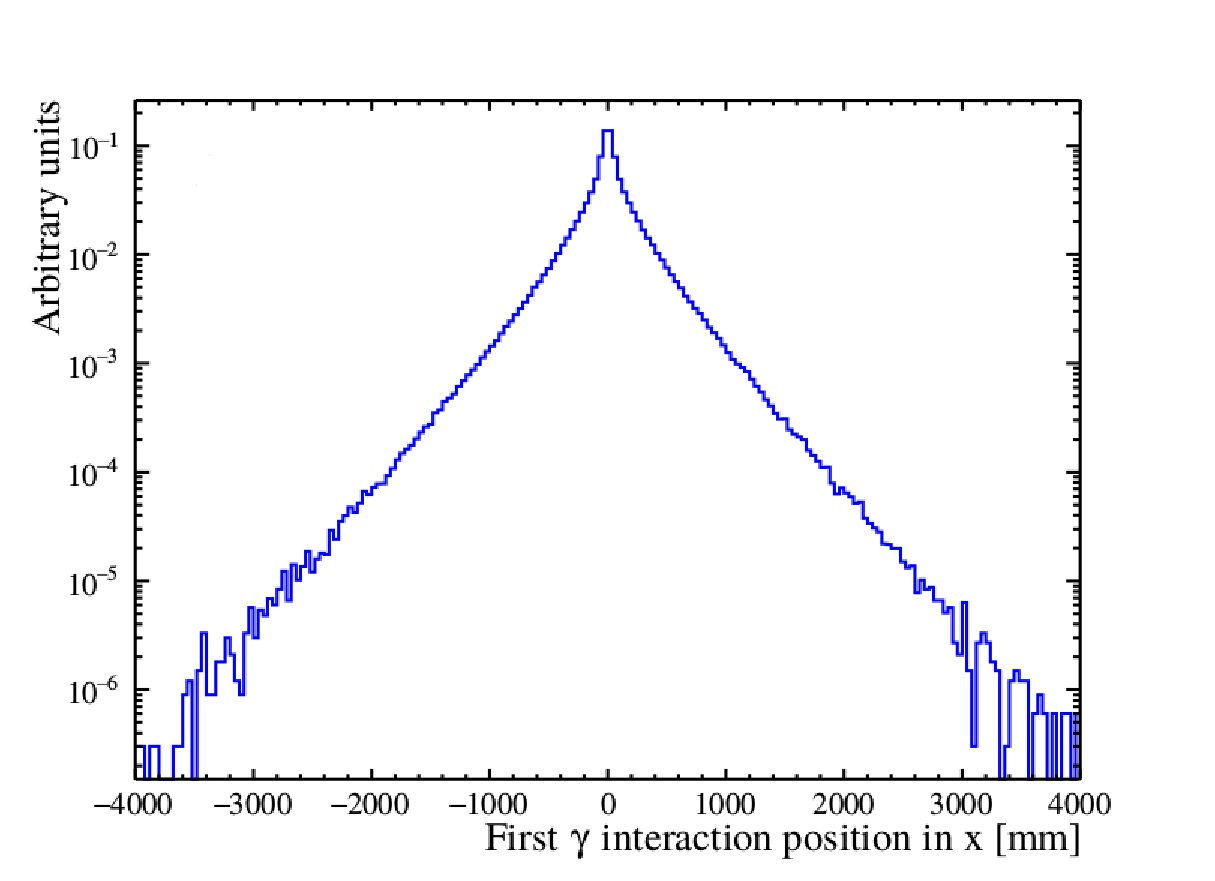
\includegraphics[width=0.79\textwidth]{gamma_first_scattering}
    \caption[Distribution of Gamma First Interaction Distance]{
    The distribution of first interaction distances for gamma ray produced
    in the $\ce{^{16}N}$ source. Produced from MC simulation and used in
    Eqn.~\eqref{eqn:n16_position_model}.}
    \label{fig:gamma_first}
\end{figure}

\begin{figure}[htbp]
\centering
    \begin{subfigure}{0.49\textwidth}
        \centering
        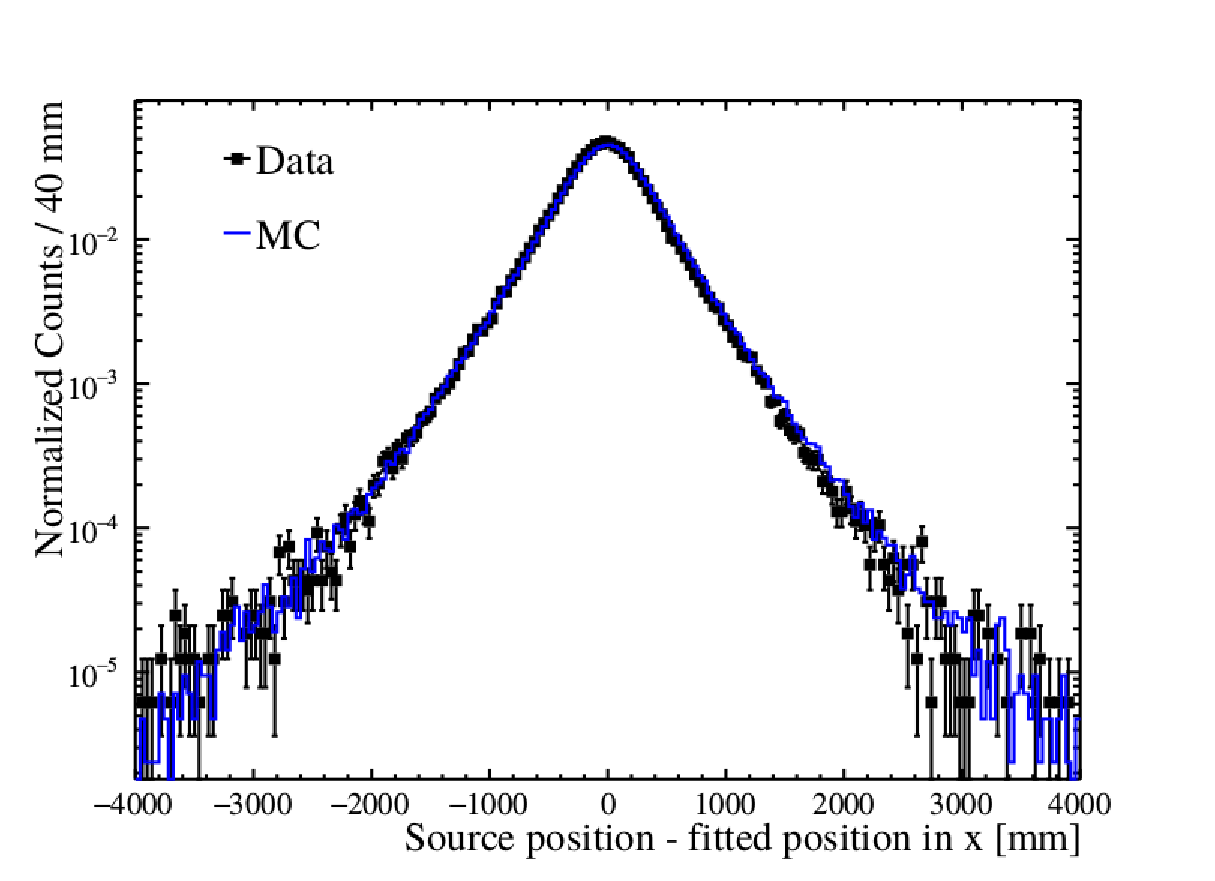
\includegraphics[width=\textwidth]{Position_data_vs_mc}
        \caption{}
    \end{subfigure}
    \begin{subfigure}{0.49\textwidth}
        \centering
        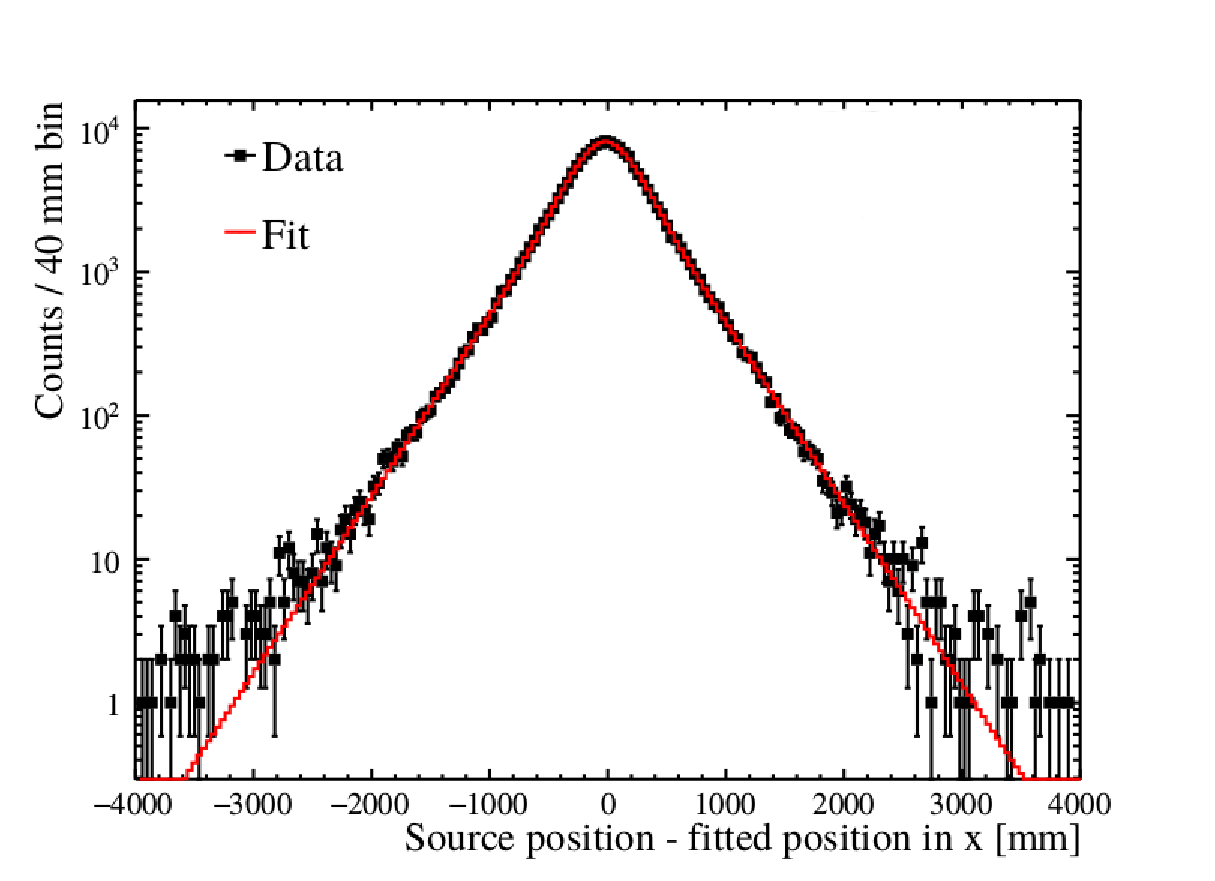
\includegraphics[width=\textwidth]{n16_position_fit_example}
        \caption{}
    \end{subfigure}
\caption[Reconstructed Postion for $\ce{^{16}N}$ events, Data and MC]{
    (a) Reconstructed position of $\ce{^{16}N}$ detected events and MC simulated
    events for a central $\ce{^{16}N}$ run. (b) An example fit to detected events,
    also for a central $\ce{^{16}N}$ run.}
\label{fig:n16_position_comparison}
\end{figure}

With this model three types of position uncertainties are considered, a shift
uncertainty, a resolution uncertainty, and a scale uncertainty.
Here a position shift is the value for $\mu$ in equation~\eqref{eqn:n16_position_model}
averaged over the entire detector volume, $\langle \mu \rangle$;
the position shift systematic then is the difference in $\langle \mu \rangle$
from MC simulation and as determined by detector data.
Rather than averaging over all source positions $\langle \mu \rangle$
is determined averaging over scans along the $x$, $y$ and $z$ axis and
so a position shift for each axial direction is determined.
Only source positions along each axis are used to avoid possible correlations
in each direction's position shift. The resulting systematic uncertainties along
each axial direction are given in table~\ref{tbl:position_shift_systs}.
\begin{table}
    \centering
    \begin{tabular}{|c|c|}
            \hline
            &$\langle \mu \rangle$ Systematic Uncertainty (mm)\\
            \hline
            x&+16.4, -18.2\\
            y&+22.3, -19.2\\
            z&+38.4, -16.7\\
            \hline
    \end{tabular}
    \caption{Position shift systematic uncertainties}
    \label{tbl:position_shift_systs}
\end{table}

The position resolution systematics is evaluated in a similar way as the position
shift systmatic, comparing values for
$\sigma^{2}$ in equation~\eqref{eqn:n16_position_model} instead of $\mu$,
but otherwise following the same procedure.
Table~\ref{tbl:position_resolution_systs} gives the extracted position resolution systematics uncertainties
in $\text{mm}$. The uncertainties are given as one-sided because a resolution uncertainty,
unlike the shift uncertainty,
can only be applied to MC simulation by applying addition smearing.
\begin{table}
    \centering
    \begin{tabular}{|c|c|}
            \hline
            &$\langle \sigma \rangle$ Systematic Uncertainty (mm)\\
            \hline
            x&104.0\\
            y&98.2\\
            z&106.2\\
            \hline
    \end{tabular}
    \caption{Position resolution systematic uncertainties}
    \label{tbl:position_resolution_systs}
\end{table}


The final position systematic considered is the position scale uncertainty,
which represents any position depended shift in $\mu$ between simulation
and data. Unlike the previous two uncertainties this systematic can effect the
number of events that would be predicted to fall within a volume if the
events are distributed uniformly throughout space. For this reason the position
scale systematic is sometimes called the fiducial volume systematic.

The position scale for simulation and data is determined by fitting the values
of $\mu$ as a function of position, along each axis, with a linear function.
The best fit slope for that line gives the position depedence of the position
shift. The value for that shift is defined to be zero at the center
of the detector. The position scale systematic can be though of as the
positional divergence introduced by the MC simulation compared to the detector
data. Table~\ref{tbl:position_scale_systs} gives the position scale systematic
uncertainty along each axis.

\begin{table}
    \centering
    \begin{tabular}{|c|c|}
            \hline
            &Position Scale Systematic Uncertainty (\%)\\
            \hline
            x&+0.91, -1.01\\
            y&+0.92, -1.02\\
            z&+0.91, -0.99\\
            \hline
    \end{tabular}
    \caption{Position scale systematic uncertainties}
    \label{tbl:position_scale_systs}
\end{table}

\subsection{Direction Calibration}
Like position and energy, the direction reconstruction is calibrated using data
from the $\ce{^{16}N}$ source. For each $\ce{^{16}N}$ event the direction
of the gamma is estimated as co-linear with the vector from the source
position to the reconstructed event position. The dot product of that vector
with the reconstructed event direction is taken, this gives the value $\cos\theta$
for that event,
\begin{equation}
    \cos\theta = \frac{\vec{p}_{\mathrm{fit}} - \vec{p}_{\mathrm{source}}}
                {\abs{\vec{p}_{\mathrm{fit}} - \vec{p}_{\mathrm{source}}}} \cdot \vec{d}_{\mathrm{fit}}\text{.}
\end{equation}
A fit is then performed to the distribution of events in $\cos\theta$ using
the model of a double exponential,
\begin{equation}
    P(\cos\theta) = \alpha\beta_{s}\frac{e^{\beta_{s}(\cos\theta -1)}}{1-e^{-\beta_{s}}} +
                    (1-\alpha)\beta_{l}\frac{e^{\beta_{l}(\cos\theta - 1)}}{1-e^{-\beta_{l}}}\text{.}
    \label{eq:direction_model}
\end{equation}
Where $\beta_{s}$ and $\beta_{l}$ represent the ``short'' and ``long'' decay constants
for the two exponentials, and $\alpha$ represents the relative
strength of the short exponential vs the long one.
This model was developed by the SNO experiment and is used here simply as an empirical
method to parameterize the distribution of events in $\cos\theta$.
It is shown in~\citep{pierre_luc_thesis} that the systematic uncertainties on the
parameters derived from~\eqref{eq:direction_model} can be transformed to a shift
in $\cos\theta$ given by,
\begin{equation}
    \cos\theta^{\prime} = 1+(\cos\theta-1)(1+\delta_{\theta})\text{,}
\end{equation}
where $\delta_{\theta}$ is the relative systematic uncertainty of $\beta_{s}$ and $\beta_{l}$.
Transformed this way the systematic uncertainty for the direction reconstruction
is given by
\begin{equation*}
    \delta_{\theta} = +0.08\text{,} -0.13\text{.}
\end{equation*}

\subsection{Trigger Efficiecy}
The trigger efficiency for this analysis is defined to be the probability that
the detector will trigger on an event as a function of the number of ``in-time''
hits produced by that event.
Here, in-time hits is the effective maximum number of hits as seen by the analog
trigger system for an event.
For each event the in-time nhit, $\tilde{n}_{100}$, is well
estimated by the maximum number of hits in a 100\,ns window within the event.
Effects from the rise-time of trigger pulses and the limited band-width of the
trigger system are applied as corrections to that simple estimate.

The trigger efficiecy is estimated in two different ways, using laserball
data, and using nhit-monitor data.
These methods disagree by a small, but non-negligible amount, the
reason for the disagreement is not well known, but the differences are taken
as a systematic uncertainty. Figure XXX shows the trigger efficiecy curves
for nhit-monitor and laserball data.

The nhit-monitor is detector calibration  process that's run periodically during
standard data taking. It simply consists of sending a variable number
of pedestal hits to the front-end, and then observing if the detector triggers
off of those hits or not. For the entierty of the dataset only channels in
crate 4 of the detector were pedestalled for the nhit-monitor.
This is one reason to prefer the trigger efficiency curve provided by laserball
data, the hits from the laserball are isotropic and present a much lower risk of
over-sampling a small number of channeles in the detector. Although all channels
in the detector are designed function identically, this is not something that
is closely monitored or tested, so it could be the case that the channels on
crate 4 are not represetative of the detector as a whole.

For runs taken after the detector threshold change discussed in Sec~\ref{XXX}
all methods agree that the trigger is 100\% efficient for $\tilde{n}_{100} > 10$;
only events with energy significantly below the analysis threshold (discussed
in Section~\ref{XXX}) will have a $\tilde{n}_{100} \le 10$, and so the discrepannt
estimates of the trigger
efficiecy do not have any effect on the solar analysis for the second trigger period.
For the first trigger period the trigger was not 100\% efficient till
$\tilde{n}_{100} \approx 23$, which is much closer to the analysis energy
threshold, and therefore uncertainties cannot be neglected.
